
\documentclass[a4paper,11pt]{article}
\usepackage[]{graphicx}
\usepackage[]{color}
%% maxwidth is the original width if it is less than linewidth
%% otherwise use linewidth (to make sure the graphics do not exceed the margin)
\makeatletter

\usepackage{geometry}
\geometry{verbose,tmargin=2cm,bmargin=2cm,lmargin=2cm,rmargin=2cm}
\usepackage{enumerate}
\usepackage[T1]{fontenc}      
\usepackage[utf8]{inputenc} 
\usepackage[francais]{babel}  
\usepackage{fancyhdr}
\usepackage{graphicx}
\usepackage{amssymb}
\usepackage{amsmath}
\pagestyle{fancy}
\selectlanguage{francais}
\setlength\parindent{0pt}

\linespread{1.1}
\usepackage{parskip} % paragraphs spacing


\newcounter{numero}
\newcommand{\exo}{\Large \vspace*{2mm}\addtocounter{numero}{1}{\bf Problème~\thenumero}\\[2mm] \normalsize}

\renewcommand{\headrulewidth}{1pt}
\fancyhead[L]{}
\fancyhead[C]{\footnotesize RES - Labo 2} 
\fancyhead[R]{\footnotesize }

\renewcommand{\footrulewidth}{1pt}
\fancyfoot[L]{}
\fancyfoot[C]{\textbf{\footnotesize Page \thepage}} 
\fancyfoot[R]{}
\thispagestyle{empty} % Pour ne pas avoir de header/footer sur la première page

\begin{document}
	
{\sc Réseau} \hfill Bastien Clément\newline 
{\tt \em https://github.com/galedric/Teaching-HEIGVD-RES-2016-Labo-02} \hfill \today \newline
\hrule
\vspace{5mm}
\noindent {\large \bf Labo 02~: Mesure des performances des entrées-sorties Java}\\[1.5mm]
\hrule
\vspace{3mm}

\section{Conditions de l'expérience}

L'objectif de ce laboratoire est de mesurer et comparer les performances d'entrées-sorties en Java. Plus spécifiquement, nous observerons les différences de performances entre la lecture-écrite byte par byte ou par bloc, ainsi que l'impact de l'utilisation des versions \emph{buffered} des flux d'entrées-sorties.

Les mesures ont été effectuées sur un Macbook Air (13-inch, Mid 2012) avec un processeur 1.8 GHz Intel Core i5, 4 GB de RAM, d'un disque SSD (aux caractéristiques inconnues) et Mac OS 10.11.

\section{Mesures}

Les graphiques ci-dessous représentent les résultats obtenus, une fois pour la lecture, une fois pour l'écriture. L'axe vertical représente le temps total nécessaire pour exécuter une mesure particulière, ainsi les valeurs les plus faibles sont les meilleures. Une taille de bloc de 0 correspond à une lecture byte par byte.\\

\begin{center}
	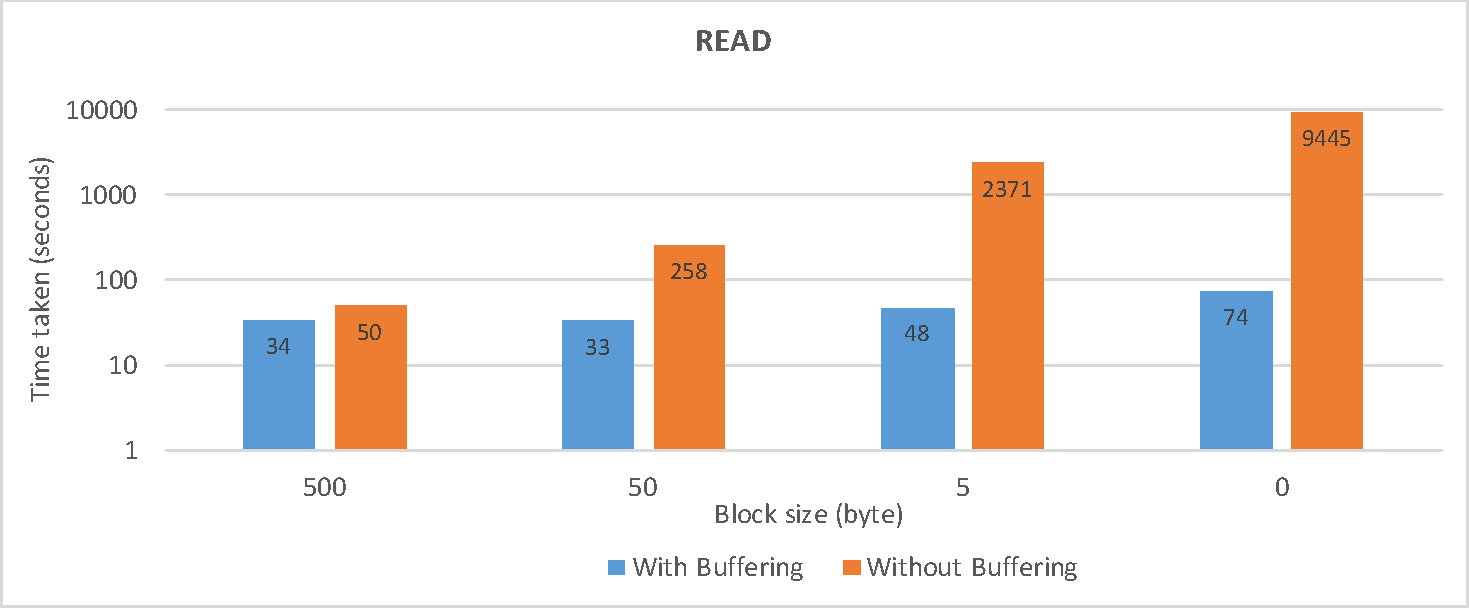
\includegraphics[width=15cm]{read}
	
	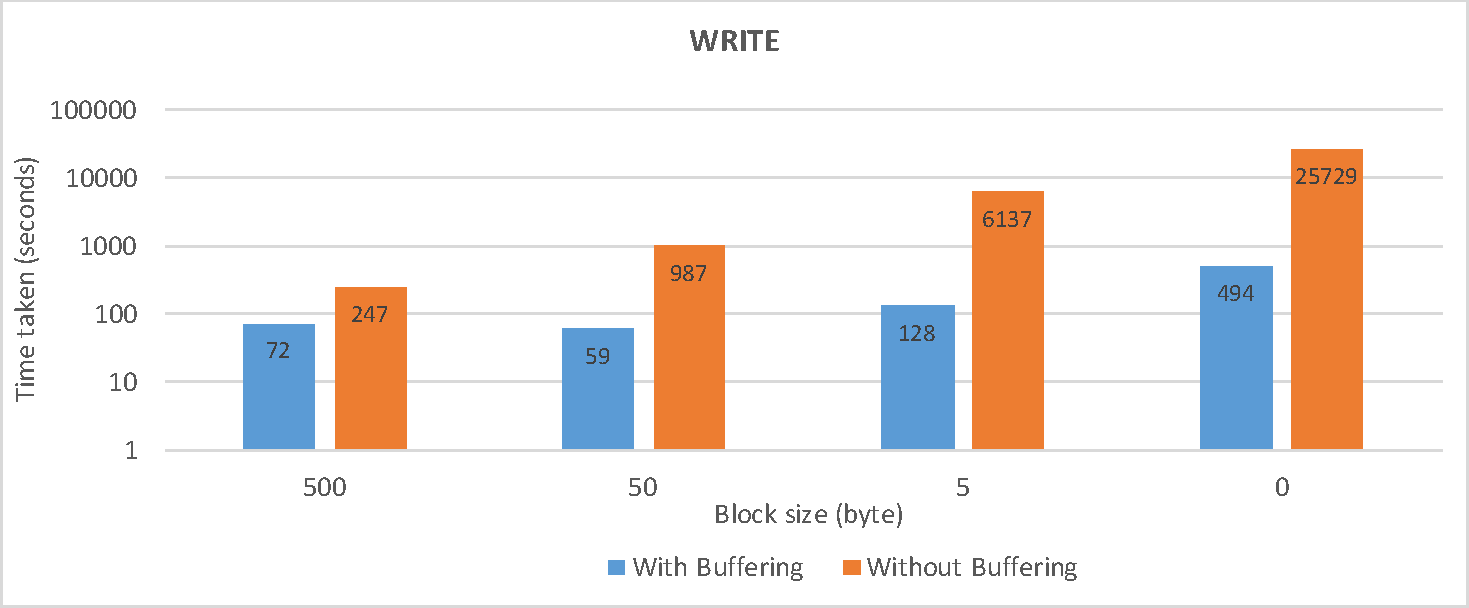
\includegraphics[width=15cm]{write}
\end{center}

\section{Analyse}

Nous observons immédiatement que l'utilisation du buffering est toujours avantageuse, que ce soit en lecture ou écriture, et indépendamment de la taille des blocs utilisée. La taille des blocs ne semble n'avoir une influence sur les performances d'entrées-sorties que lorsque nous utilisons des flux sans buffering. Avec buffering, la taille des blocs influe considérablement moins sur les performances. La raison est probablement que le buffering est en pratique équivalent à la lecture par plus gros blocs.

Malgré cela, et particulièrement pour l'écriture, l'utilisation d'entrées-sorties byte par byte semble sensiblement plus coûteuse que les entrées-sorties par blocs, et ceci même avec utilisation du buffering. J'imagine que le temps supplémentaire est probablement dépensé dans la JVM. En effet il n'y a pas de raison que la fréquence des appels système de lecture ou d'écriture soient différents puisque le flux utilise de toute façon des lectures par blocs, de même pour les performances d'entrées-sorties du disque. À l'inverse, la lecture byte par byte implique un nombre beaucoup plus important d'itérations de la boucle de lecture/écriture et d'appels de fonction dans le programme Java.

Il me parait aussi important de noter que la méthodologie utilisée lors des mesures de performances ne me semble tout à fait rigoureuse. Premièrement, seul 10 MB sont lus ou écrits. Les temps mesurés sont de quelques millisecondes. À cette échelle, une petite perturbation due aux processus parallèles sur le système peuvent représenter une variation relativement importante sur la mesure. Effectuer les test avec des fichiers plus gros serait probablement une bonne idée. De même, la mesure n'est effectuée qu'une seule fois, pour plus de précision, réitérer l'expérience conduirait à des résultats plus fiables.

Finalement, les mécanismes de cache du système de fichier et du noyau ne sont pas du tout considérés. En pratique, la lecture d'un fichier qui vient d'être écrit (tel que c'est le cas dans ce laboratoire) peut probablement être effectuée directement depuis les caches du système de fichier, sans accès réel au disque. Cela ne semble cependant pas être le cas ici.

\section{Explications}

Afin de générer le fichier \texttt{.csv}, j'ai choisi une implémentation simple et directe, sans particulièrement me soucier de la réutilisabilité du code écrit.

Ainsi j'ai implémenté deux classes \texttt{TestResult} et \texttt{TestOutputBuilder}.

\texttt{TestResult} représente les résultats d'un test spécifique. C'est un bête conteneur de valeurs sans aucune méthode, c'est pourquoi j'ai choisi de déclarer tous les attributs \texttt{public static final} au lieu d'utiliser des getters. Ce modèle est inspiré des \emph{case class} du langage Scala.

\texttt{TestOutputBuilder} est un objet construit avec comme paramètre un \texttt{OutputStream} dans lequel les données CSV textuelles doivent être écrites. Sa méthode \texttt{headers(String ...headers)} permet de spécifier une ligne d'en-têtes à écrire sur le flux de sortie avant les premier résultats. La méthode \texttt{add(TestResult r)} permet d'écrire une ligne sur le flux de sortie, correspondant au résultat d'un test en particulier. Finalement la méthode \texttt{close()} ferme le flux sous-jacent et vide ainsi tous les tampons entre le flux haut-niveau et le fichier sur le disque.

Lors de la construction de l'objet \texttt{TestOutputBuilder} dans la fonction \texttt{main}, j'ai également décoré mon \texttt{FileOutputStream} avec un \texttt{BufferedOutputStream}, puisque comme le test a pu le montré, les performances sont supérieures à celles d'un flux non décoré.

J'ai également choisi de modifier le type de retour de certaines fonctions afin de faire remonter les résultats des tests jusque dans la fonction principale.

\end{document}